%adding TAIGA|Tunka data

% 11. Присоединение данных TAIGA (Tunka-133, HiSCORE) (как идея)
%         отличие тунки от каскада, черенки/сцинтиляторы
%         картинки с хмах
%         мэппинг данных
%
%         разделение гамма/кр тунка133 +

\begin{frame}{Tunka-133 and TAIGA HiScore}
\begin{minipage}[c]{0.49\textwidth}
\begin{itemize}
  \item TAIGA setups are located at the latitude as KASCADE;
  \item The possibility to scale  Tunka-133 and KASCADE-Grande was shown at:
  W.D.~Apel et al., \textit{Tunka-Rex and LOPES Collaborations}, Phys.\ Lett.\ B \textbf{763} (2016) 179
\end{itemize}
\end{minipage}
\hfill
\begin{minipage}[c]{0.49\textwidth}
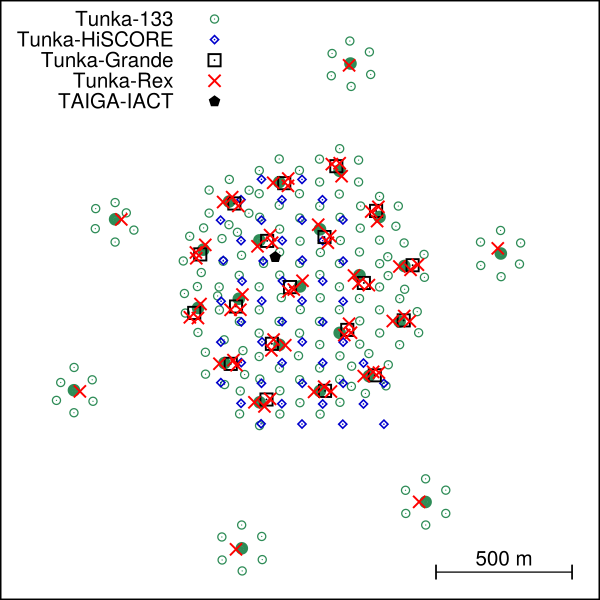
\includegraphics[width=1\textwidth]{pics/taiga_map.png}
\end{minipage}
% A comparison of the cosmic-ray energy scales of Tunka-133 and
% KASCADE-Grande via their radio extensions Tunka-Rex and LOPES
\end{frame}


\begin{frame}{KASCADE-TAIGA joint analysis}
\small
\begin{center}
    \begin{minipage}{0.55\textwidth}
     	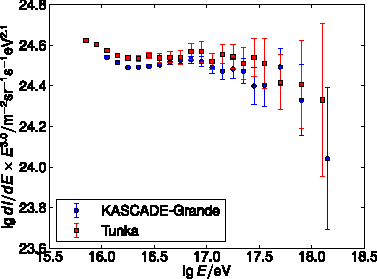
\includegraphics[width=1\textwidth]{pics/KG_tunka133_scales.pdf}
    \end{minipage}
%     \begin{minipage}{0.07\textwidth}
     $\longleftarrow$ 
%     \end{minipage}
\begin{minipage}{0.38\textwidth}	
  Energy spectra of cosmic rays from KASCADE-Grande and Tunka-133: normalized flux per energy.
\end{minipage}
\end{center}

\begin{itemize}
 \item  With a systematic increase of
KASCADE-Grande energies by 4\% (or a corresponding decrease of Tunka-133 energies) 
the average flux per energy of both experiments can be brought to agreement
in this energy range.
\end{itemize}
% \end{minipage}
\end{frame}

\begin{frame}{Tunka-133 $\gamma$-proton separation}
\begin{minipage}[c]{0.49\textwidth}
  \begin{center}
    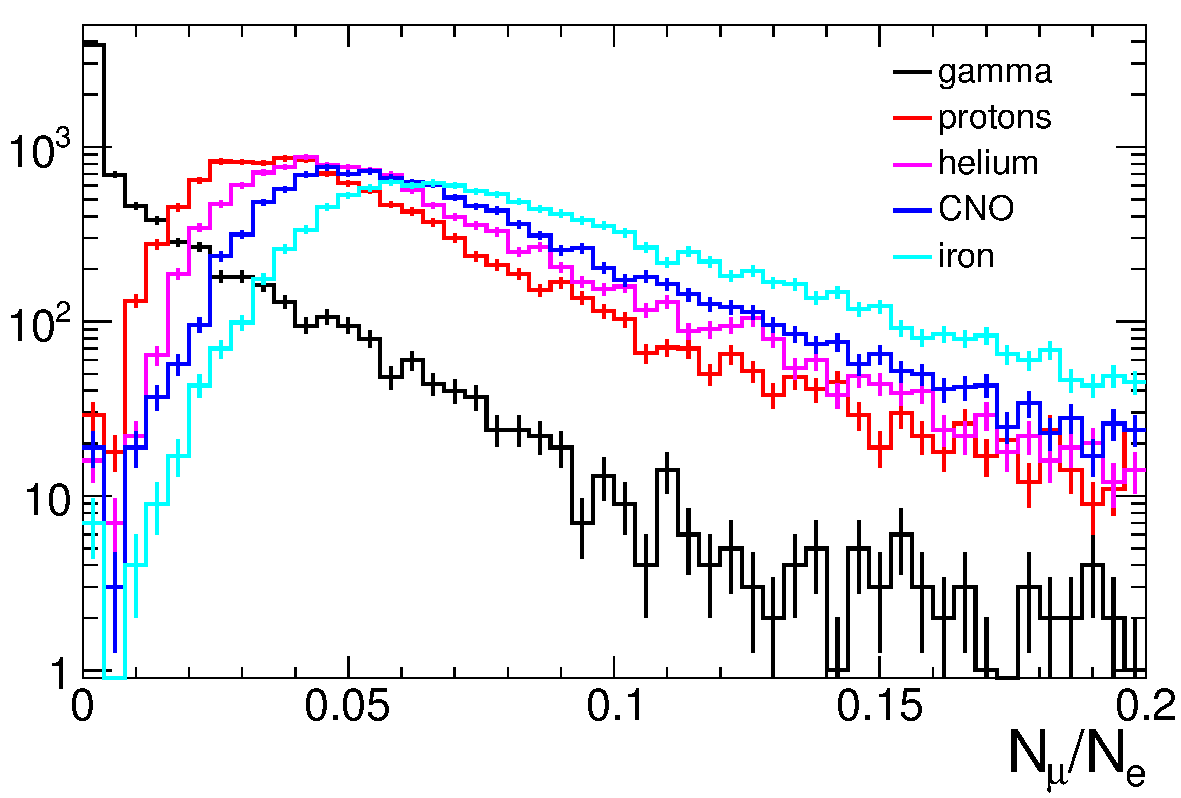
\includegraphics[width=1\textwidth]{pics/Nmu_Ne.pdf}\\
    Distribution of $N_\mu / N_e$ for various primary CR components for KASCADE.
  \end{center}
\end{minipage}
\hfill
\begin{minipage}[c]{0.49\textwidth}
  \begin{center}
    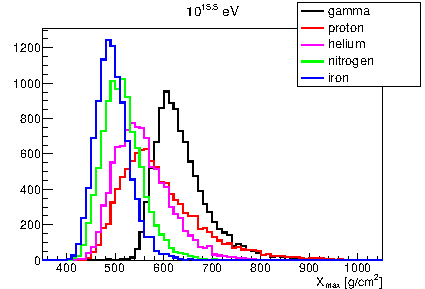
\includegraphics[width=1\textwidth]{pics/tunka_gamma_cr_diff.pdf}\\
    Distribution of $X_{max}$ for various primary CR components at $E = 10^{15.5}$~eV for Tunka-133.
  \end{center}
\end{minipage}
\vspace{1ex}
\begin{itemize}
  \item $X_{max}$ alone is not sufficient for $\gamma$-proton separation.
  \item It is essential to use scintillation counters with the ability of electron-muon discrimination, installed at Tunka-Grande.
\end{itemize}
\end{frame}
